\chapter{状態、測定、複素ベクトル空間}

\lectureoverview{量子力学は、状態という言葉の意味を変えることから始まる。まず古典論における状態と決定論的更新のパターンを抽出し、次に二つの結果をもつスピン実験を用いてその破綻を明らかにする。これに対する数学的な応答は、双対ベクトル、内積、ノルム、直交性を備えた複素ベクトル空間である。}

\section{古典的なパターン：状態と更新}

まず閉じた系を考える。少なくとも一時的には他のすべてから孤立しているものとする。ここで\emph{系}という語は原始的である。すなわち、その履歴を予測したい対象を意味する。\emph{状態}とは、その予測を行うためにある瞬間に知られていなければならないすべてのことである。古典力学は、一つの状態を次の状態へと更新する法則を与える。

最も単純な抽象的なコインに対しては、
\begin{equation}
  \mathcal S_{\mathrm{coin}}=\{H,T\}.
\end{equation}
一つの可能な法則は、何も起こらないというものである：
\begin{equation}
  H\longmapsto H,
  \qquad
  T\longmapsto T.
\end{equation}
別の法則は二つの状態を交互に入れ替える：
\begin{equation}
  H\longmapsto T,
  \qquad
  T\longmapsto H.
\end{equation}
これらの例は初歩的であるが、古典論の構造を明らかにする：
\begin{equation}
  s(t)\longmapsto s(t+\Delta t).
\end{equation}
ひとたび\(s(t)\)が分かれば、更新は決定論的である。

状態空間が連続的であっても、同じパターンは保たれる。直線上を運動する粒子には、その位置と運動量の両方が必要であり、
\begin{equation}
  s=(q,p),
\end{equation}
したがってその状態空間は相平面である。可能な状態の数は無限になり、方程式はラグランジアン、ハミルトニアン、ポアソン括弧という洗練された言葉で書かれるかもしれないが、根底にある考え方は変わっていない。ある時刻の状態は、別の時刻の状態を予測するために必要なものを含んでいる。

\section{可視化の前に抽象化}

古典的な運動は、その概念が日常経験から引き出されているため、比較的思い描きやすい。しかし、対象が小さすぎたり、速度が大きすぎたり、状態空間の次元が高すぎたりすると、その利点は失われる。電子の運動、四次元時空、あるいは十次元空間を文字通り思い描く人はいない。これは初学者に特有の欠陥ではない。人間の視覚的直観は、日常的な三次元世界のために作られたのである。

一見単純な場合でも、この限界は現れる。二次元の曲がった空間の絵と呼ばれるものは、通常、三次元に埋め込まれた曲面である。一次元の直線は、平面内の印として思い描かれる。その絵は、我々の視覚系が操作する方法を知っている周囲の空間を、密かに持ち込んでいるのである。

救済策は、古典的な絵をなじみのない物理学に無理に当てはめることではない。抽象的な構造を学び、正しい操作から新しい直観を育てることである。三次元座標\((x,y,z)\)は、記号を一つ加えて規則を拡張することにより四次元座標\((x,y,z,w)\)になるのであって、新たな視覚器官を獲得することによるのではない。量子力学も同じ規律を要求する。それを小さな古典的対象の奇妙な力学模型として扱えば、繰り返し誤った答えを生むことになる。

\begin{remark}
数学的直観は依然として発達する。それは単に、海の波や通常の空間における矢印を見ることと同じではないだけである。その関係が一貫して用いられるため、代数はなじみ深いものになる。
\end{remark}

\section{古典的状態空間と古典論理}

古典系では、状態空間は集合である。抽象的なサイコロは
\begin{equation}
  \mathcal S_{\mathrm{die}}=\{1,2,3,4,5,6\}.
\end{equation}
を持つ。実在のサイコロは連続的に多くの向きをもつが、ここで用いる理想化されたサイコロはこれらの六つのラベルだけをもつ。直線上の粒子は連続的に無限の集合
\begin{equation}
  \mathcal S_{\mathrm{particle}}
  =
  \{(q,p)\mid q,p\in\mathbb R\}.
\end{equation}
をもつ。有限であれ無限であれ、各々の古典的状態空間は互いに異なる可能性の集まりである。

系についての命題は、それらの可能性の部分集合を選び出す。サイコロに対して、
\begin{align}
  P_{\mathrm{odd}}&=\{1,3,5\},\\
  P_{\leq 3}&=\{1,2,3\}.
\end{align}
としよう。\emph{奇数かつ三以下}という文は、それらの共通部分に対応する：
\begin{equation}
  P_{\mathrm{odd}}\cap P_{\leq 3}=\{1,3\}.
\end{equation}
\emph{奇数または三以下}という包括的な文は、それらの和集合に対応する：
\begin{equation}
  P_{\mathrm{odd}}\cup P_{\leq 3}
  =
  \{1,2,3,5\}.
\end{equation}
したがって、古典的な論理積と論理和は集合論的な形
\begin{equation}
  P\wedge Q\longleftrightarrow P\cap Q,
  \qquad
  P\vee Q\longleftrightarrow P\cup Q.
\end{equation}
をもつ。部分集合が重ならないならば、両方の命題を真にする状態は存在しない。

この論理は、状態についての古典的な概念と結びついている。量子力学は、古典的な選択肢の集合を、別の数学的対象、すなわちベクトル空間に置き換える。ベクトル空間による記述が、排他的な配置の集合のように近似的に振る舞うのは、適切な古典的極限においてのみである。その空間を構成する前に、この置き換えを避けられなくする実験が必要である。

\section{最も単純な量子系}

抽象的なコインの量子版は、\emph{qubit} と呼ばれる二結果系である。その測定される選択肢には、まず表と裏というラベルを付けてもよいが、数値ラベルの方がより有用である：
\begin{equation}
  \sigma\in\{+1,-1\}.
\end{equation}
三つの記法を並行して用いる：
\begin{equation}
  H\longleftrightarrow \sigma=+1\longleftrightarrow\uparrow,
  \qquad
  T\longleftrightarrow \sigma=-1\longleftrightarrow\downarrow.
\end{equation}
最初のうち、矢印は単なる名前である。通常の幾何学的ベクトルはまだ仮定されていない。

\begin{figure}[htbp]
  \centering
  \includegraphics[width=0.78\textwidth]{lecture_01_figure_02.png}
  \caption{この板書では、等価なラベル \(H/T\)、\(\sigma=\pm1\)、および上向き／下向きの矢印を導入する。矢印は記法として始まるのであり、古典的模型としてではない。}
  \lectureframe{00:22:44}
\end{figure}

\begin{classroomqa}
\audiencequestion{表と裏は物理系とどのような関係があるのか。}
\lecturerresponse{二つの親しみやすい名前を与える以外には何もない。qubit はこの測定に対して二つの可能な結果をもち、表と裏は仮の名にすぎない。ラベル \(\pm1\) は方程式に入れることができるため選ばれている。}
\end{classroomqa}

\subsection{黒箱としての装置}

実験には第二の系、すなわち装置 \(A\) が必要である。今のところ、それは三つの特徴をもつ抽象的な黒箱である：
\begin{enumerate}
  \item 空間的な向きをもち、\emph{this side up} によって示される；
  \item qubit と相互作用できるセンサーをもつ；
  \item 最初は空白であり、その後 \(+1\) または \(-1\) を表示するディスプレイをもつ。
\end{enumerate}
検出器の詳細は意図的に後回しにする。良い検出器は、系とその記録との間の信頼できる関係によって操作的に定義される。相互作用が起こるときに観測者が見ている必要はない；装置は結果を記録し、後で読み出せる。

ディスプレイが \(+1\) を報告したとしよう。装置を空白状態にリセットし、独立な発展が作用する時間がないうちに、直ちに同じ測定を繰り返す。忠実な検出器は再び \(+1\) を報告する。最初の結果が \(-1\) ならば、直ちに繰り返しても同様に \(-1\) を報告し続ける：
\begin{equation}
\begin{aligned}
  +1&\longrightarrow +1\longrightarrow +1\longrightarrow\cdots,\\
  -1&\longrightarrow -1\longrightarrow -1\longrightarrow\cdots.
\end{aligned}
\end{equation}
したがって、最初の測定は\emph{準備}と見なすことができる。それは qubit を、同じ測定を直ちに繰り返すと確定した結果をもつような状態に残す。

この再現性は、任意の哲学的注釈ではない。これがなければ、測定を確認する操作的な方法は存在しない。欠陥のある装置はその結果を再現できないかもしれないが、その場合それは、定義されている理想的な測定を行っているのではない。

\begin{classroomqa}
\audiencequestion{これはすでに波動関数の収縮なのか。}
\lecturerresponse{その言葉は後で導入できる。この段階では、操作的な記述で十分である：測定は結果を生み、同じ即時測定がその結果を再現するような状態を準備する。その過程に名前を付けても、まだそれを説明したことにはならない。}
\end{classroomqa}

\section{向きと古典的ポインターの失敗}

正立した装置が \(+1\) を読むように qubit を準備する。装置を \(180^\circ\) 回転させ、測定を繰り返す。結果は今度は \(-1\) である。反転した装置での繰り返し測定は \(-1\) を確認し、装置を再び正立させると \(+1\) が回復する。

この結果は真正の方向性を明らかにする。上向き／下向きの記法は完全に任意ではない：検出器を反転すると符号が反転する。qubit は単に小さなベクトルであり、検出器はそのベクトルの自身の軸に沿った成分を測定している、と結論したくなる。その誘惑は信じるのではなく検証されなければならない。

\begin{figure}[htbp]
  \centering
  \includegraphics[width=0.82\textwidth]{lecture_01_figure_03.png}
  \caption{上向きの準備と、板上の異なる向きの分析器。教室では後にチョークの矢印の一つが訂正された；議論では分析器の軸だけが重要である。}
  \lectureframe{00:36:21}
\end{figure}

\subsection{横向きの測定}

検出器を \(90^\circ\) 回転させる。準備された qubit が通常の上向きポインターならば、水平な検出器軸に沿ったその成分はゼロであろう：
\begin{equation}
  \hat{\mathbf x}\cdot\hat{\mathbf z}=0.
\end{equation}
量子装置は決してゼロを報告しない。各試行は常に \(+1\) または \(-1\) のいずれかを報告する。

\begin{figure}[htbp]
  \centering
  \resizebox{\linewidth}{!}{%
  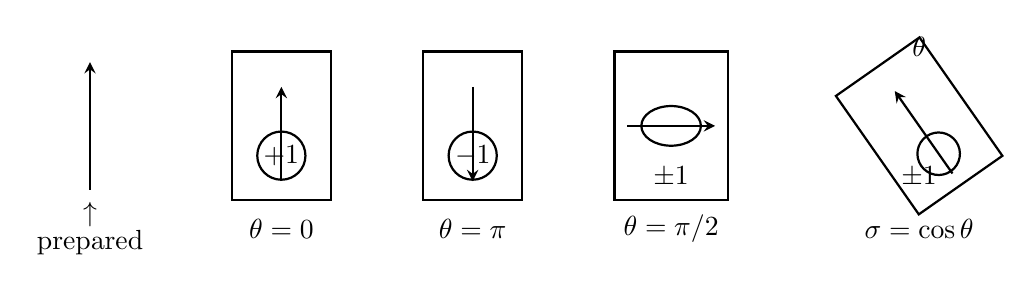
\begin{tikzpicture}[>=stealth,thick,scale=0.90]
    \draw[->] (0,0)--(0,1.8);
    \node at (0,-0.35) {\(\uparrow\)};
    \node at (0,-0.75) {prepared};

    \draw (2.0,-0.15) rectangle (3.4,1.95);
    \draw (2.7,0.48) circle (0.34);
    \draw[->] (2.7,0.12)--(2.7,1.45);
    \node at (2.7,0.48) {\(+1\)};
    \node at (2.7,-0.55) {\(\theta=0\)};

    \draw (4.7,-0.15) rectangle (6.1,1.95);
    \draw (5.4,0.48) circle (0.34);
    \draw[->] (5.4,1.45)--(5.4,0.12);
    \node at (5.4,0.48) {\(-1\)};
    \node at (5.4,-0.55) {\(\theta=\pi\)};

    \draw (7.4,-0.15) rectangle (9.0,1.95);
    \draw (8.2,0.90) ellipse (0.42 and 0.28);
    \draw[->] (7.58,0.90)--(8.82,0.90);
    \node at (8.2,0.18) {\(\pm1\)};
    \node at (8.2,-0.55) {\(\theta=\pi/2\)};

    \begin{scope}[shift={(11.7,0.90)},rotate=35]
      \draw (-0.72,-1.02) rectangle (0.72,1.02);
      \draw (0,-0.48) circle (0.30);
      \draw[->] (0,-0.82)--(0,0.60);
    \end{scope}
    \node at (11.7,0.18) {\(\pm1\)};
    \node at (11.7,-0.55) {\(\expect{\sigma}=\cos\theta\)};
    \node at (11.7,2.02) {\(\theta\)};
  \end{tikzpicture}
  }%
  \caption{分析器列の再構成。回転は統計を変えるが、個々の結果の集合は決して変えない。}
\end{figure}

正立した装置で qubit の大きな集団を準備し、結果が \(+1\) であるものを保持する。保持された各 qubit を横向きの装置で一度測定する。試行の半数は \(+1\) を与え、半数は \(-1\) を与え、アンサンブル平均はゼロである：
\begin{equation}
  \expect{\sigma}_{\pi/2}=0.
\end{equation}
平均は古典的ポインターの消える水平成分に似ているが、個々の記録はそうではない。古典的な値 \(0\) は、二つの離散的な結果の間の統計的釣り合いに置き換えられている。

\begin{classroomqa}
\audiencequestion{同じ量子ビットを横向き測定の後に捨てずに保持し続けると、何が起こるか。}
\lecturerresponse{その最初の横向きの結果が\(+1\)であるとしよう。同じ量子ビットに対して横向き測定を繰り返すと、\(+1\)が何度も得られる。最初の横向き測定は、その量子ビットを横向き軸に対して準備したのである。五十対五十の統計を得るには、一つの結果を繰り返し確認するのではなく、準備と測定の実験全体を多数の量子ビットに対して繰り返さなければならない。}
\end{classroomqa}

\subsection{両立しない準備}

軸の順序が重要である。\(+1\)を縦向きに準備し、次に横向きに測定する。最初の横向きの結果はランダムである。一度横向きの結果が得られると、直ちに横向きを繰り返すと結果は確定している。次に検出器を縦向き軸に戻す。縦向きの結果は再びランダムになる。

記号で書けば、\(M_z\)と\(M_x\)が二つの軸に沿った測定を表すとき、
\begin{equation}
\begin{aligned}
  M_z&:+1,\\
  M_x&:\pm1,\\
  M_x&:\text{same result},\\
  M_z&:\pm1.
\end{aligned}
\end{equation}
中間の\(x\)測定は、元の縦向き状態を保ったまま横向き成分を露わにしただけではない。それは新しい状態を準備し、元の縦向きの確定性は失われている。

\begin{classroomqa}
\audiencequestion{検出器は最初の答えを覚えているのか。同じ量子ビットが提示されたのか新しい量子ビットが提示されたのかを、どうやって知ることができるのか。}
\lecturerresponse{繰り返し性は測定された量子ビットの性質であり、検出器が行う隠れた記憶の比較ではない。測定の後、量子ビットは同じ即時測定に対して同じ答えを与える状態にある。異なる準備をされた量子ビットを提示すれば、結果はその準備に依存する。どの物理系が測定されているかを追跡することは、通常の実験室での記録管理である。}
\end{classroomqa}

\begin{classroomqa}
\audiencequestion{では、観測という行為がその特定の量子ビットを準備するのか。}
\lecturerresponse{そのとおりである。その測定が量子ビットを準備してしまえば、何か他の発展や両立しない測定が介在しない限り、同じ測定は同じ答えを与える。}
\end{classroomqa}

\section{任意の角度に回転した分析器}

検出器の軸が、集団が準備された軸と角度\(\theta\)をなすものとする。各試行は依然として
\begin{equation}
  \sigma=\pm1.
\end{equation}
を与える。相対頻度は角度とともに変化し、平均は
\begin{equation}
  \expect{\sigma}_{\theta}=\cos\theta.
  \label{eq:qml1-cosine-mean}
\end{equation}
となる。極限的な場合は
\begin{align}
  \expect{\sigma}_{0}&=+1,\\
  \expect{\sigma}_{\pi/2}&=0,\\
  \expect{\sigma}_{\pi}&=-1.
\end{align}
である。\(\theta=0\)の近くでは、ほとんどの結果は\(+1\)であり、時折\(-1\)が現れる。\(\theta=\pi\)の近くでは、ほとんどは\(-1\)であり、時折\(+1\)が現れる。

\begin{figure}[htbp]
  \centering
  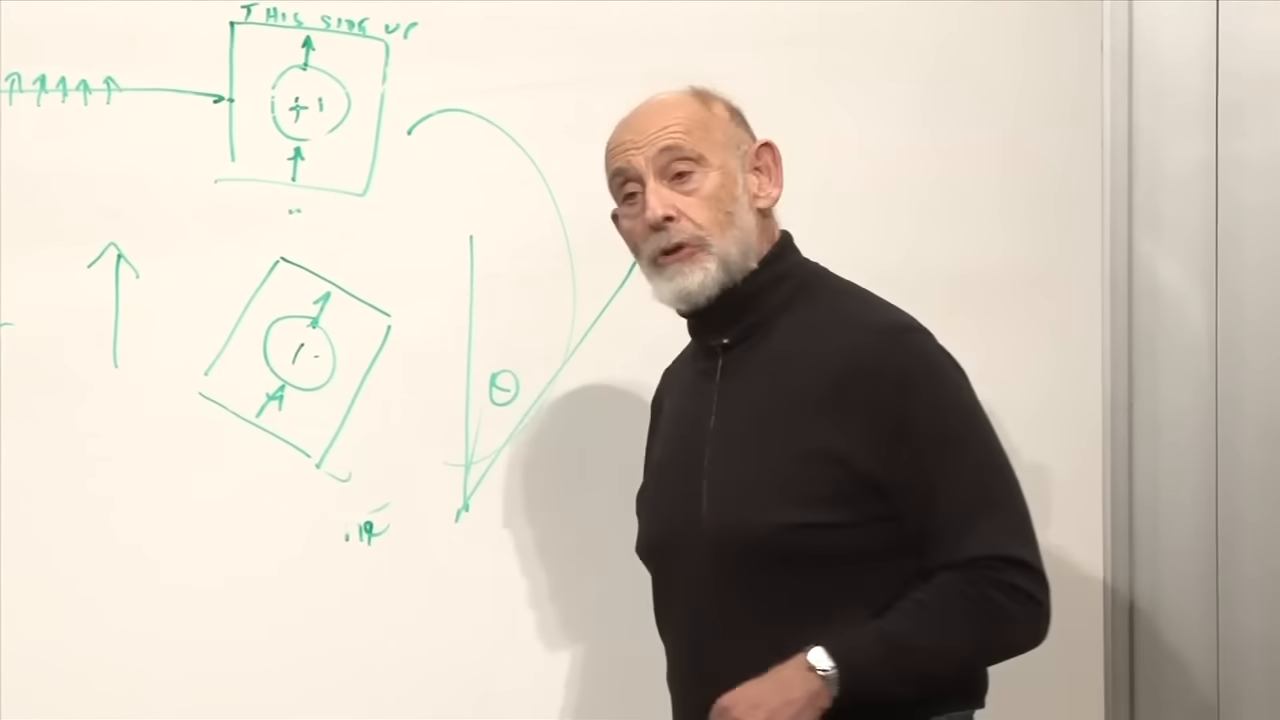
\includegraphics[width=0.82\textwidth]{lecture_01_figure_04.png}
  \caption{任意角度の実験の実際の板書：縦向きに準備された集団が、\(\theta\)だけ傾いた分析器に入る。}
  \lectureframe{00:48:55}
\end{figure}

滑らかなベクトル的な量は集団平均であり、単一の結果ではない。\(p_+(\theta)\)と\(p_-(\theta)\)が二つの確率であるならば、
\begin{equation}
  p_+ + p_-=1,
  \qquad
  p_+-p_-=\cos\theta.
\end{equation}
したがって、
\begin{equation}
\begin{aligned}
  p_+(\theta)&=\frac{1+\cos\theta}{2}
  =\cos^2\frac{\theta}{2},\\
  p_-(\theta)&=\frac{1-\cos\theta}{2}
  =\sin^2\frac{\theta}{2}.
\end{aligned}
  \label{eq:qml1-half-angle-probabilities}
\end{equation}
\editorialnote{講義は二つの結果とその平均\(\cos\theta\)を述べている。式~\eqref{eq:qml1-half-angle-probabilities}はそれらの記述から直ちに導かれる代数的帰結であり、暗黙の頻度法則を明示するものである。}

\begin{classroomqa}
\audiencequestion{準備されていない量子ビットの集まりも\(\cos\theta\)の平均を示すだろうか。}
\lecturerresponse{偏りのない集まりでは特定の方向が選ばれていないので、その平均はゼロである。\(\theta\)依存性は、まず確定した軸に沿って準備された集団を指している。}
\end{classroomqa}

\begin{classroomqa}
\audiencequestion{量子ビットに介在する力学が何もないのなら、なぜ集団全体が必要なのか。}
\lecturerresponse{一つの量子ビットに対する最初の傾いた測定は一つの標本を与える。同じ量子ビットに対する即時の繰り返しはすべて、その標本を確認するだけである。独立な試行には、同一に準備された量子ビットが必要であり、それぞれが傾いた分析器で一度だけ測定される。}
\end{classroomqa}

\begin{classroomqa}
\audiencequestion{プラスとマイナスの並びにパターンや高次の相関はあるのか。}
\lecturerresponse{この実験では、個々の試行は独立で無相関であるとみなす。それらの一回試行の確率は\(\theta\)に依存するが、追加の順序パターンは主張していない。}
\end{classroomqa}

\subsection{理想化された点}

当面、装置は連続的に調整可能な向きと離散的な読み出しをもつ古典的物体として扱う。この\emph{系}と\emph{検出器}の分割は一時的なものである。検出器自身も物理系であり、最終的には量子力学に従わなければならない。完全な説明は系と装置を一緒に扱うことになるが、それにはまだ利用できない道具立てが必要である。

\begin{classroomqa}
\audiencequestion{検出器それ自体もまた、ただの二状態系にすぎないのだろうか。}
\lecturerresponse{検出器には物理的状態があり、最終的には量子論的記述に含めなければならない。当面は操作上の分割を保つ。すなわち、量子ビットは量子力学的に記述される対象であり、向きづけられた検出器は安定した古典的記録を与える。後に、結合系を相互作用する量子系として解析しなければならない。}
\end{classroomqa}

\begin{classroomqa}
\audiencequestion{検出器を回転させる軸を変えると、ここに示した単一の角度よりも多くの構造が導入されるのだろうか。}
\lecturerresponse{はい、完全な三次元の話はより豊かである。一平面内の回転はその最も単純な断面であり、後に述べるより完全な取り扱いと整合している。}
\end{classroomqa}

\begin{classroomqa}
\audiencequestion{検出器は\(-1\)と\(+1\)の間の連続的な値を返すことができるのだろうか。}
\lecturerresponse{その向きは連続的に変化するが、各理想的な量子ビット読み出しは依然として\(+1\)または\(-1\)である。連続性は、向きが変化するにつれて確率と平均に現れるのであって、個々の結果に現れるのではない。}
\end{classroomqa}

\section{ポインターと抽象ベクトル}

ここでしばらく、実験的事実と数学を切り離す。物理空間における通常の矢印を\emph{ポインター}と呼ぶ。数学的なベクトルはより一般的である。すなわち、それはベクトル空間の元であり、通常の空間内のどこかを指す必要はない。

\begin{definition}
複素ベクトル空間\(V\)とは、ベクトルの和と複素スカラーによる乗法が定義され、通常の線形性の規則を満たすようなベクトルの集まりである。特に、\(u,v,w\in V\)および\(a,b\in\mathbb C\)に対して、
\begin{align}
  u+v&=v+u,\\
  (u+v)+w&=u+(v+w),\\
  a(u+v)&=au+av,\\
  (a+b)u&=au+bu,\\
  (ab)u&=a(bu),\\
  1u&=u.
\end{align}
零ベクトル\(0\)が存在し、各\(u\)に対して加法逆元\(-u\)が存在する。
\end{definition}

教室での議論では、最初は演算と閉性のみを強調する。
\begin{equation}
\begin{aligned}
  u,v\in V&\Longrightarrow u+v\in V,\\
  a\in\mathbb C,\ u\in V&\Longrightarrow au\in V.
\end{aligned}
\end{equation}
零ベクトルと可換性は、その後、質問への応答として与えられる。残りのよく知られた公理は、具体的な列ベクトル模型を導入するときにすでに用いられているものを明示的に述べたものである。

実数は\(\mathbb R\)上の一次元ベクトル空間をなす。複素数は\(\mathbb C\)上の一次元ベクトル空間をなし、\(\mathbb R\)上の二次元ベクトル空間をなす。複素数値関数\(\psi(x)\)もまた複素ベクトル空間をなす。なぜなら
\begin{equation}
  (\psi+\phi)(x)=\psi(x)+\phi(x),
  \qquad
  (z\psi)(x)=z\psi(x).
\end{equation}
この関数空間の例は後に中心的になるが、有限の列のほうがまず構造を見やすい。

\begin{classroomqa}
\audiencequestion{ベクトルとベクトル空間の区別は何か。}
\lecturerresponse{ベクトルは一つの元である。ベクトル空間は、そのような元すべての集まりであり、それらを加えたりスカラー倍したりする規則を伴う。ちょうど、数は一つの対象であり、数体系は演算を伴う集まりであるのと同じである。}
\end{classroomqa}

\section{二成分複素列}

抽象ベクトルをディラック記法で\(\ket{\alpha}\)と書く。具体的な表現は
\begin{equation}
  \ket{\alpha}
  \longleftrightarrow
  \begin{pmatrix}
    \alpha_1\\
    \alpha_2
  \end{pmatrix},
  \qquad
  \alpha_1,\alpha_2\in\mathbb C.
\end{equation}
もし
\begin{equation}
  \ket{\beta}
  \longleftrightarrow
  \begin{pmatrix}
    \beta_1\\
    \beta_2
  \end{pmatrix},
\end{equation}
ならば、加法とスカラー乗法は成分ごとに定義される。
\begin{align}
  \ket{\alpha}+\ket{\beta}
  &\longleftrightarrow
  \begin{pmatrix}
    \alpha_1+\beta_1\\
    \alpha_2+\beta_2
  \end{pmatrix},\\
  z\ket{\alpha}
  &\longleftrightarrow
  \begin{pmatrix}
    z\alpha_1\\
    z\alpha_2
  \end{pmatrix},
  \qquad z\in\mathbb C.
\end{align}

\begin{figure}[htbp]
  \centering
  \includegraphics[width=0.88\textwidth]{lecture_01_figure_05.png}
  \caption{二つの複素列を加え、一つの列を複素スカラー倍するための成分ごとの規則。}
  \lectureframe{01:14:28}
\end{figure}

零ベクトルは
\begin{equation}
  \ket{0}
  =
  \begin{pmatrix}
    0\\
    0
  \end{pmatrix},
  \qquad
  \ket{\alpha}+\ket{0}=\ket{\alpha}.
\end{equation}
長さ三の列は別のベクトル空間をなし、任意の固定された長さについても同様である。二成分の列を三成分の列に加えることはできない。なぜなら、両者は異なる空間に属し、それらを関係づける成分ごとの規則が存在しないからである。

\begin{classroomqa}
\audiencequestion{列ベクトルは行列なのだろうか。}
\lecturerresponse{一般的な用語では、それは一列の行列である。この講義では、\emph{行列}という語は通常、正方配列を意味し、一列の配列は列ベクトルと呼ばれる。この区別は用語上のものであり、代数についての見解の相違ではない。}
\end{classroomqa}

\begin{classroomqa}
\audiencequestion{ベクトルの加法の順序は重要だろうか。}
\lecturerresponse{いいえ。成分ごとの加法は複素数の可換性を受け継ぐ。
\[
  \ket{\alpha}+\ket{\beta}
  =
  \ket{\beta}+\ket{\alpha}.
\]
これはベクトル空間の公理の一つである。}
\end{classroomqa}

\section{双対ベクトル：ブラとケット}

各ケット\(\ket{A}\)に対して、双対空間内に対応するベクトルが存在し、\(\bra{A}\)と書く。ケットからブラへの写像は加法的であるが、複素スカラーを複素共役にする。
\begin{align}
  \ket{A}+\ket{B}
  &\longleftrightarrow
  \bra{A}+\bra{B},\\
  z\ket{A}
  &\longleftrightarrow
  z^*\bra{A}.
  \label{eq:qml1-antilinear-dual}
\end{align}
この第二の規則が本質的な複素的特徴である。スカラー倍の双対は、複素共役スカラーを掛けたものになる。

\begin{figure}[htbp]
  \centering
  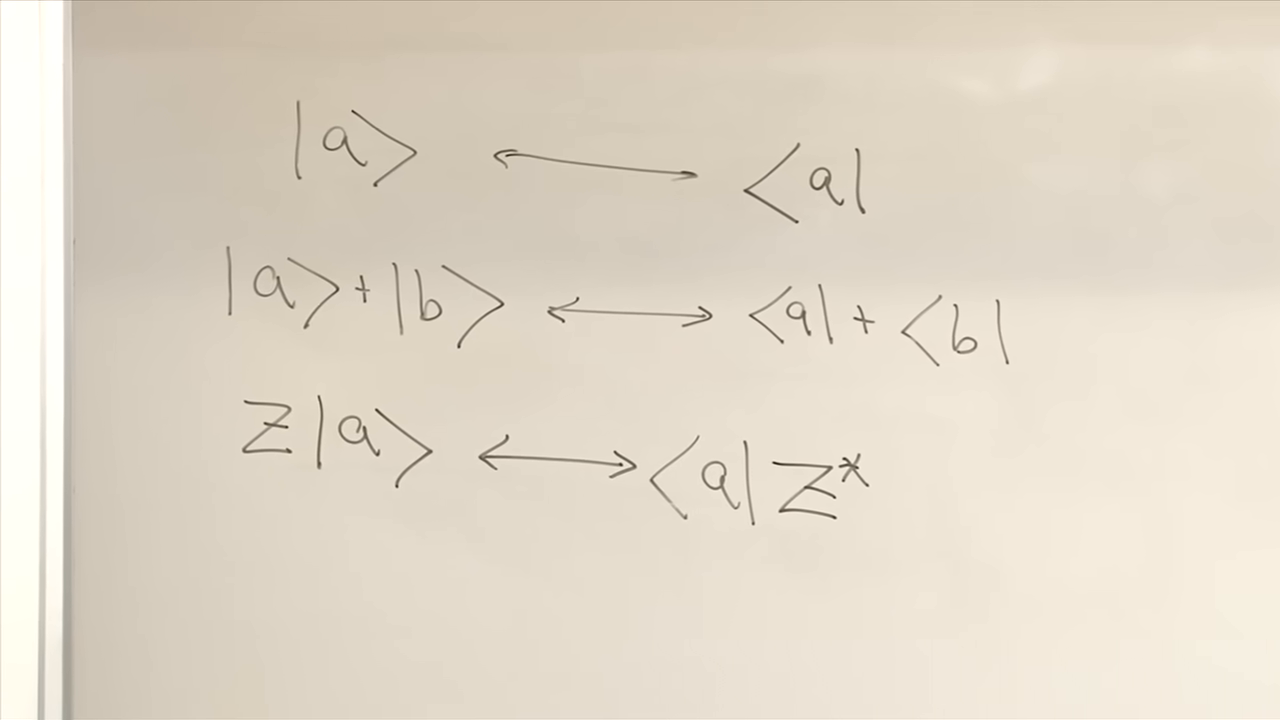
\includegraphics[width=0.86\textwidth]{lecture_01_figure_06.png}
  \caption{ケットからブラへの対応とその二つの規則：和は和に写り、スカラー乗法は複素共役をとる。}
  \lectureframe{01:23:15}
\end{figure}

2成分表示では、
\begin{equation}
  \ket{\alpha}
  =
  \begin{pmatrix}
    \alpha_1\\
    \alpha_2
  \end{pmatrix}
  \qquad\Longrightarrow\qquad
  \bra{\alpha}
  =
  \begin{pmatrix}
    \alpha_1^*&\alpha_2^*
  \end{pmatrix}.
  \label{eq:qml1-bra-from-ket}
\end{equation}
複素共役が双対対応を実現し、行記法によって2種類の対象が目に見えて区別される。式~\eqref{eq:qml1-bra-from-ket}は式~\eqref{eq:qml1-antilinear-dual}を直接検証するものでもある。

\section{内積}

\(\ket{\alpha}\)と\(\ket{\beta}\)が与えられたとき、\(\beta\)に対応するbraとket\(\alpha\)を組み合わせる：
\begin{equation}
  \braket{\beta}{\alpha}
  =
  \begin{pmatrix}
    \beta_1^*&\beta_2^*
  \end{pmatrix}
  \begin{pmatrix}
    \alpha_1\\
    \alpha_2
  \end{pmatrix}
  =
  \beta_1^*\alpha_1+\beta_2^*\alpha_2.
  \label{eq:qml1-inner-product}
\end{equation}
\emph{bracket}という語は、文字通り\emph{bra}と\emph{ket}から組み立てられている。これはドット積の複素類似物である：対応する成分を掛けて足し合わせ、bra側では複素共役をとる。

\begin{figure}[htbp]
  \centering
  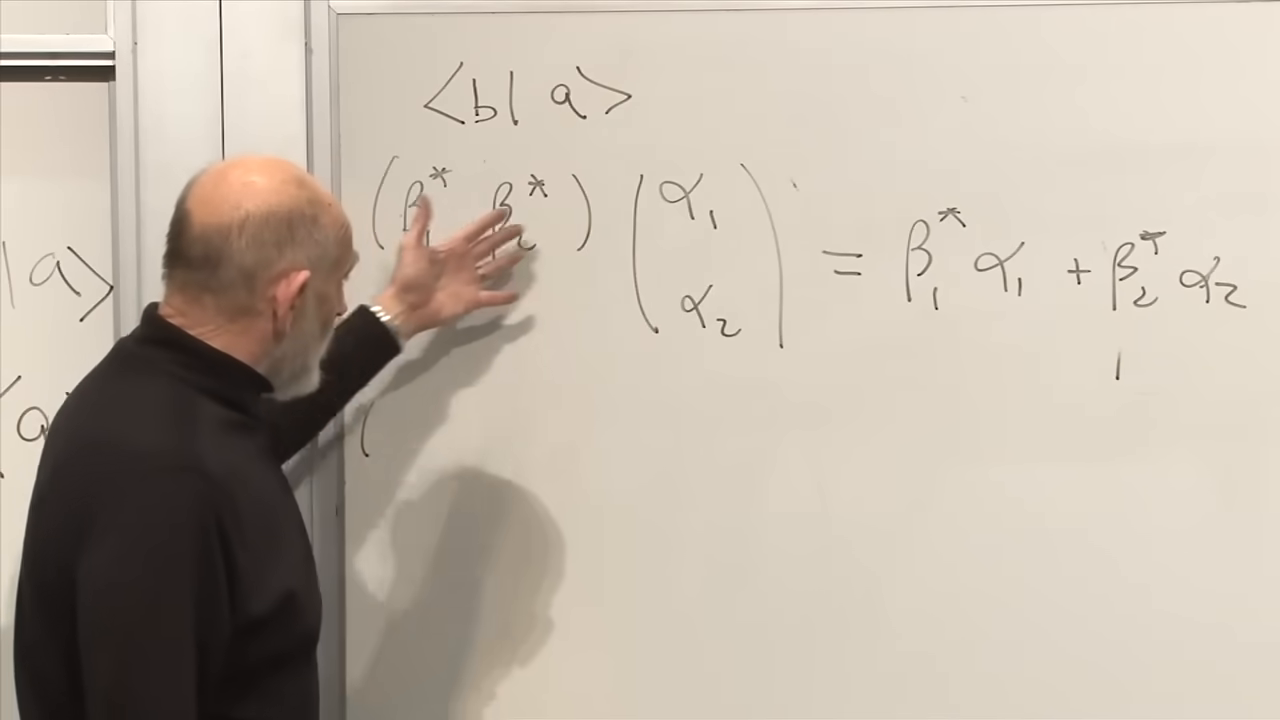
\includegraphics[width=0.88\textwidth]{lecture_01_figure_07.png}
  \caption{黒板では内積\(\braket{\beta}{\alpha}\)を\(\beta_1^*\alpha_1+\beta_2^*\alpha_2\)と評価する。}
  \lectureframe{01:31:25}
\end{figure}

ベクトルを入れ替えると
\begin{equation}
  \braket{\alpha}{\beta}
  =
  \alpha_1^*\beta_1+\alpha_2^*\beta_2
  =
  \braket{\beta}{\alpha}^{*}.
  \label{eq:qml1-conjugate-symmetry}
\end{equation}
したがって一般には順序が重要であるが、その違いは複素共役だけである。

\begin{classroomqa}
\audiencequestion{片側を共役せずに複素ベクトルの積を定義できるだろうか。}
\lecturerresponse{そのような双線形な表式を発明することはできるが、その場合ベクトル自身との積が実数や正である必要はない。その構造は量子力学に有用なものではない。共役をとった、すなわちエルミート内積が、後に必要となるノルムと確率の構造を与える。}
\end{classroomqa}

\subsection{ノルムと正値性}

式~\eqref{eq:qml1-inner-product}で\(\beta=\alpha\)と置く：
\begin{equation}
  \braket{\alpha}{\alpha}
  =
  \alpha_1^*\alpha_1+\alpha_2^*\alpha_2
  =
  |\alpha_1|^2+|\alpha_2|^2.
  \label{eq:qml1-norm-square}
\end{equation}
この数は自身の複素共役に等しいので実数である。これは非負であり、零ベクトルのときのみ消える。長さは
\begin{equation}
  \|\alpha\|
  =
  \sqrt{\braket{\alpha}{\alpha}}.
\end{equation}
で定義される。したがって複素成分から通常の非負実数の長さが得られる。

\begin{figure}[htbp]
  \centering
  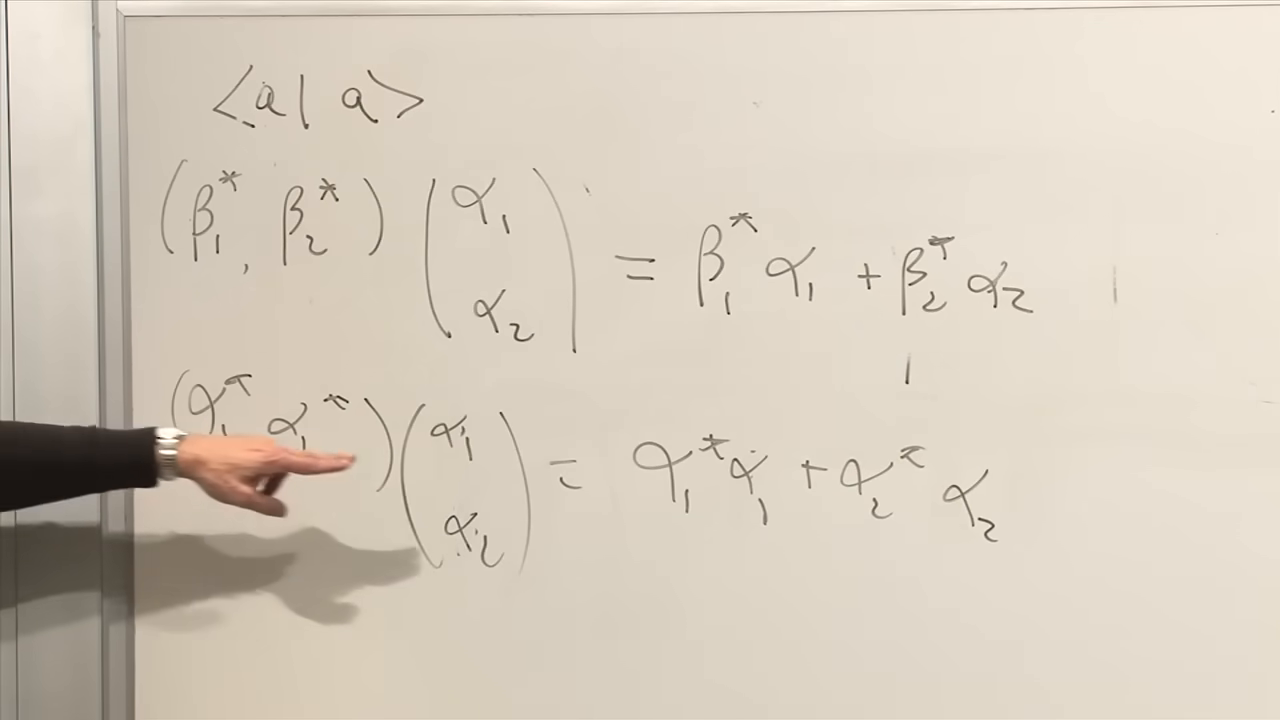
\includegraphics[width=0.88\textwidth]{lecture_01_figure_08.png}
  \caption{ボード上の自己内積：\(\braket{\alpha}{\alpha}=|\alpha_1|^2+|\alpha_2|^2\)、すなわちノルムの二乗である。}
  \lectureframe{01:34:40}
\end{figure}

\section{直交性と次元}

2つのベクトルは、その内積が消えるとき直交する：
\begin{equation}
  \braket{\beta}{\alpha}=0.
  \label{eq:qml1-orthogonality}
\end{equation}
共役対称性により、この関係は順序に依存しない：
\begin{equation}
  \braket{\beta}{\alpha}=0
  \quad\Longrightarrow\quad
  \braket{\alpha}{\beta}
  =
  \braket{\beta}{\alpha}^{*}
  =0.
\end{equation}

2成分空間では、最も単純な直交対は
\begin{equation}
  \ket{e_1}
  =
  \begin{pmatrix}
    1\\
    0
  \end{pmatrix},
  \qquad
  \ket{e_2}
  =
  \begin{pmatrix}
    0\\
    1
  \end{pmatrix},
  \qquad
  \braket{e_1}{e_2}=0.
  \label{eq:qml1-standard-basis}
\end{equation}

\begin{figure}[htbp]
  \centering
  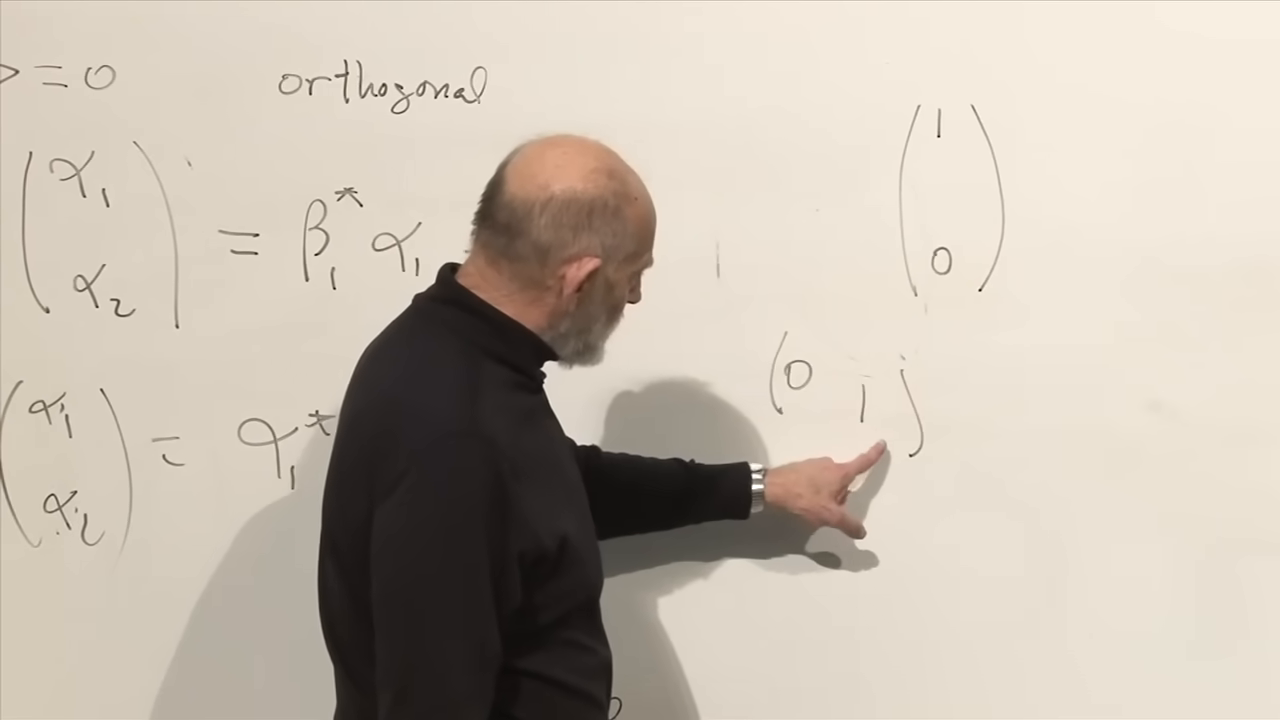
\includegraphics[width=0.88\textwidth]{lecture_01_figure_09.png}
  \caption{黒板では標準的な直交列\((1,0)^{\mathsf T}\)と\((0,1)^{\mathsf T}\)を構成する。}
  \lectureframe{01:39:50}
\end{figure}

次元は、互いに直交する非零ベクトルの最大個数として特徴づけられる。2次元空間ではそのようなベクトルは2個あり得るが、3個目はない。これを具体的に見るために、
\begin{equation}
  \ket{v}
  =
  \begin{pmatrix}
    v_1\\
    v_2
  \end{pmatrix}
\end{equation}
が式~\eqref{eq:qml1-standard-basis}の両方のベクトルに直交するとする。すると
\begin{equation}
  \braket{e_1}{v}=v_1=0,
  \qquad
  \braket{e_2}{v}=v_2=0,
\end{equation}
なので\(\ket{v}=\ket{0}\)である。両方に直交する3個目の非零ベクトルは存在しない。

\begin{classroomqa}
\audiencequestion{零ベクトルはすべてのベクトルに直交するので、余分な1個を与えるのではないか。}
\lecturerresponse{その通りである。だからこそ定義では\emph{非零}の互いに直交するベクトルと言わなければならない。零ベクトルは独立な方向を持たず、次元を数える際には除外される。}
\end{classroomqa}

\begin{remark}
列表示では、次元は成分の数に等しい。直交性の定義はより抽象的であり、すでに座標を選んでいることに依存しない。
\end{remark}

\section{黒板でのさらなる質問}

\begin{classroomqa}
\audiencequestion{同じ構造は関数のベクトル空間にも当てはまるか。}
\lecturerresponse{はい。関数は、連続的に添字づけられた成分\(\psi(x)\)をもつ列とみなせる。加法とスカラー倍は各点ごとである。対応する内積は有限和ではなく積分になる；その構成は後に展開される。}
\end{classroomqa}

\begin{classroomqa}
\audiencequestion{ketにbraを掛けると行列が得られるか。}
\lecturerresponse{はい。内積\(\bra{\beta}\ket{\alpha}\)は行と列を縮約して数を与える。順序を逆にした\(\ket{\alpha}\bra{\beta}\)は外積、すなわち正方行列を与える。内積と外積はどちらも重要になる。}
\end{classroomqa}

\begin{classroomqa}
\audiencequestion{測定はqubitを単に明らかにするのではなく、実際に影響を与えるのか。}
\lecturerresponse{はい。新しい軸に沿った最初の測定は新しい状態を準備する。だからこそ、その測定を繰り返すと答えが確認され、古い軸に戻ると不確定性が復活する。この不可避の擾乱が、原理的にはいくらでも穏やかに行える理想化された古典測定と量子実験を区別する。}
\end{classroomqa}

\section{構成の二つの半分}

ここで、まだ結び付けられていない二つの半分が手元にある。実験の半分はこう述べる：
\begin{enumerate}
  \item 理想的な量子ビット測定の結果は\(\pm1\)のみである；
  \item 同じ即時測定を繰り返すと結果が確認される；
  \item 検出器の軸を変えると、測定によって準備される状態が変わる；
  \item 準備された集団に対して、\(\theta\)だけ傾けた分析器の平均は\(\cos\theta\)である。
\end{enumerate}
数学の半分はこう述べる：
\begin{enumerate}
  \item 量子状態は古典的な点ではなくベクトルで表される；
  \item 関係するベクトルは複素ベクトル空間をなす；
  \item ケットには双対のブラがあり、ブラは複素スケーリングの下で反線形に作用する；
  \item エルミート内積が長さ、直交性、次元を定義する。
\end{enumerate}

次の課題は、これらの半分を結び付けることである。量子ビットの二次元複素状態空間は、分析器実験の再現性、ランダム性、角度依存の統計を再現しなければならない。量子力学が始まるのは、何か隠れた古典的描像ではなく、まさにこの結び付きにおいてである。
